% =====================================================================
% Figure 1 — BowTie diagram (TikZ-native)
%
% Generated as vector graphics inside the document; no external file
% needed. Loaded into Section 4 via % =====================================================================
% Figure 1 — BowTie diagram (TikZ-native)
%
% Generated as vector graphics inside the document; no external file
% needed. Loaded into Section 4 via % =====================================================================
% Figure 1 — BowTie diagram (TikZ-native)
%
% Generated as vector graphics inside the document; no external file
% needed. Loaded into Section 4 via % =====================================================================
% Figure 1 — BowTie diagram (TikZ-native)
%
% Generated as vector graphics inside the document; no external file
% needed. Loaded into Section 4 via \input{figs/fig1_bowtie.tex}.
% =====================================================================

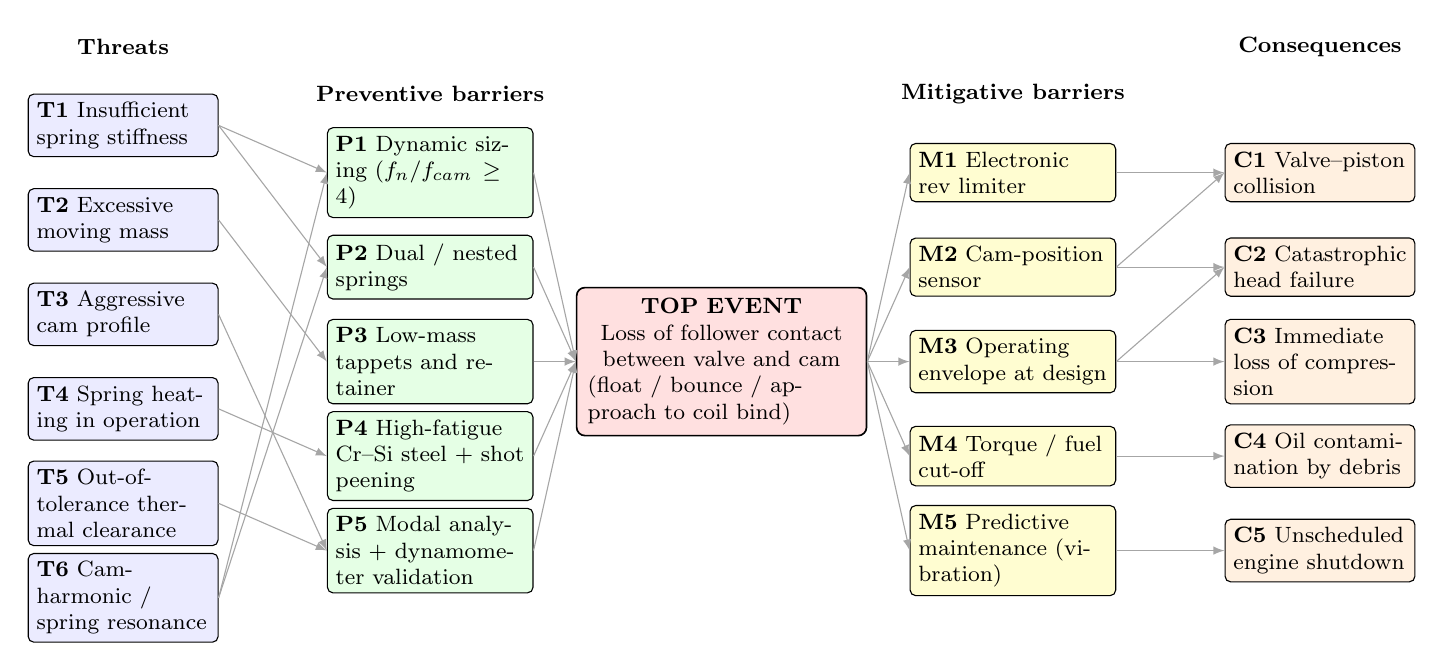
\begin{tikzpicture}[
  font=\footnotesize,
  every node/.style={align=left},
  threat/.style={draw,fill=blue!8,rounded corners=2pt,inner sep=3pt,minimum width=22mm,minimum height=6mm,text width=22mm},
  pbar/.style={draw,fill=green!10,rounded corners=2pt,inner sep=3pt,minimum width=24mm,minimum height=6mm,text width=24mm},
  cons/.style={draw,fill=orange!12,rounded corners=2pt,inner sep=3pt,minimum width=22mm,minimum height=6mm,text width=22mm},
  mbar/.style={draw,fill=yellow!18,rounded corners=2pt,inner sep=3pt,minimum width=24mm,minimum height=6mm,text width=24mm},
  topev/.style={draw,fill=red!12,line width=0.6pt,rounded corners=3pt,inner sep=4pt,minimum width=34mm,minimum height=12mm,text width=34mm},
  flow/.style={->,>=latex,line width=0.4pt,gray!70},
]

% ---- Top event (centre)
\node[topev] (TE) at (0,0)
  {\centering\textbf{TOP EVENT}\\Loss of follower contact between valve and cam\\(float / bounce / approach to coil bind)};

% ---- Threats (left, T1..T6)
\node[threat] (T1) at (-7.6, 3.0) {\textbf{T1} Insufficient spring stiffness};
\node[threat] (T2) at (-7.6, 1.8) {\textbf{T2} Excessive moving mass};
\node[threat] (T3) at (-7.6, 0.6) {\textbf{T3} Aggressive cam profile};
\node[threat] (T4) at (-7.6,-0.6) {\textbf{T4} Spring heating in operation};
\node[threat] (T5) at (-7.6,-1.8) {\textbf{T5} Out-of-tolerance thermal clearance};
\node[threat] (T6) at (-7.6,-3.0) {\textbf{T6} Cam-harmonic / spring resonance};

% ---- Preventive barriers (between threats and TE)
\node[pbar] (P1) at (-3.7, 2.4) {\textbf{P1} Dynamic sizing ($f_n/f_{cam}\geq 4$)};
\node[pbar] (P2) at (-3.7, 1.2) {\textbf{P2} Dual / nested springs};
\node[pbar] (P3) at (-3.7, 0.0) {\textbf{P3} Low-mass tappets and retainer};
\node[pbar] (P4) at (-3.7,-1.2) {\textbf{P4} High-fatigue Cr--Si steel + shot peening};
\node[pbar] (P5) at (-3.7,-2.4) {\textbf{P5} Modal analysis + dynamometer validation};

% ---- Consequences (right, C1..C5)
\node[cons] (C1) at (7.6, 2.4) {\textbf{C1} Valve--piston collision};
\node[cons] (C2) at (7.6, 1.2) {\textbf{C2} Catastrophic head failure};
\node[cons] (C3) at (7.6, 0.0) {\textbf{C3} Immediate loss of compression};
\node[cons] (C4) at (7.6,-1.2) {\textbf{C4} Oil contamination by debris};
\node[cons] (C5) at (7.6,-2.4) {\textbf{C5} Unscheduled engine shutdown};

% ---- Mitigative barriers (between TE and consequences)
\node[mbar] (M1) at (3.7, 2.4) {\textbf{M1} Electronic rev limiter};
\node[mbar] (M2) at (3.7, 1.2) {\textbf{M2} Cam-position sensor};
\node[mbar] (M3) at (3.7, 0.0) {\textbf{M3} Operating envelope at design};
\node[mbar] (M4) at (3.7,-1.2) {\textbf{M4} Torque / fuel cut-off};
\node[mbar] (M5) at (3.7,-2.4) {\textbf{M5} Predictive maintenance (vibration)};

% ---- Threats -> Preventive barriers (many-to-some mapping)
\draw[flow] (T1.east) -- (P1.west);
\draw[flow] (T2.east) -- (P3.west);
\draw[flow] (T3.east) -- (P5.west);
\draw[flow] (T4.east) -- (P4.west);
\draw[flow] (T5.east) -- (P5.west);
\draw[flow] (T6.east) -- (P1.west);
\draw[flow] (T1.east) -- (P2.west);
\draw[flow] (T6.east) -- (P2.west);

% ---- Preventive barriers -> Top event
\draw[flow] (P1.east) -- (TE.west);
\draw[flow] (P2.east) -- (TE.west);
\draw[flow] (P3.east) -- (TE.west);
\draw[flow] (P4.east) -- (TE.west);
\draw[flow] (P5.east) -- (TE.west);

% ---- Top event -> Mitigative barriers
\draw[flow] (TE.east) -- (M1.west);
\draw[flow] (TE.east) -- (M2.west);
\draw[flow] (TE.east) -- (M3.west);
\draw[flow] (TE.east) -- (M4.west);
\draw[flow] (TE.east) -- (M5.west);

% ---- Mitigative barriers -> Consequences
\draw[flow] (M1.east) -- (C1.west);
\draw[flow] (M2.east) -- (C1.west);
\draw[flow] (M3.east) -- (C2.west);
\draw[flow] (M3.east) -- (C3.west);
\draw[flow] (M4.east) -- (C4.west);
\draw[flow] (M5.east) -- (C5.west);
\draw[flow] (M2.east) -- (C2.west);

% ---- Side labels
\node[font=\footnotesize\bfseries] at (-7.6, 4.0) {Threats};
\node[font=\footnotesize\bfseries] at (-3.7, 3.4) {Preventive barriers};
\node[font=\footnotesize\bfseries] at ( 3.7, 3.4) {Mitigative barriers};
\node[font=\footnotesize\bfseries] at ( 7.6, 4.0) {Consequences};

\end{tikzpicture}
.
% =====================================================================

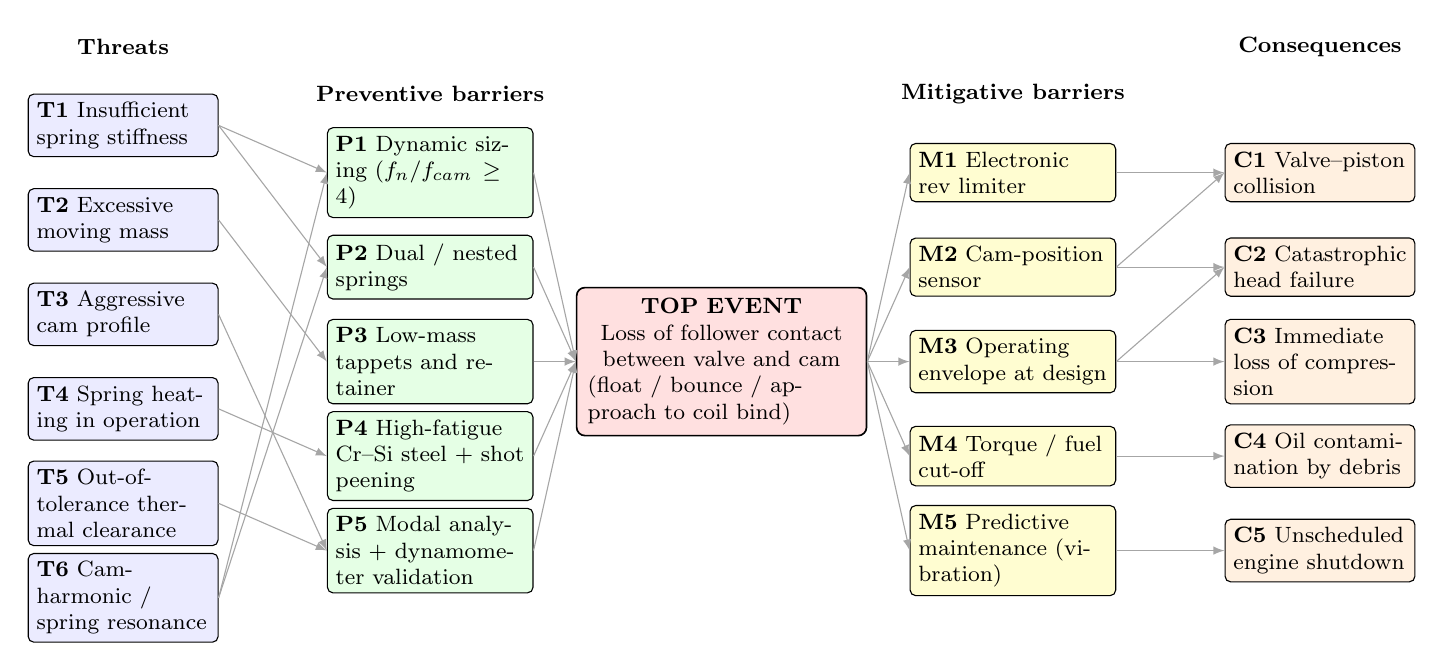
\begin{tikzpicture}[
  font=\footnotesize,
  every node/.style={align=left},
  threat/.style={draw,fill=blue!8,rounded corners=2pt,inner sep=3pt,minimum width=22mm,minimum height=6mm,text width=22mm},
  pbar/.style={draw,fill=green!10,rounded corners=2pt,inner sep=3pt,minimum width=24mm,minimum height=6mm,text width=24mm},
  cons/.style={draw,fill=orange!12,rounded corners=2pt,inner sep=3pt,minimum width=22mm,minimum height=6mm,text width=22mm},
  mbar/.style={draw,fill=yellow!18,rounded corners=2pt,inner sep=3pt,minimum width=24mm,minimum height=6mm,text width=24mm},
  topev/.style={draw,fill=red!12,line width=0.6pt,rounded corners=3pt,inner sep=4pt,minimum width=34mm,minimum height=12mm,text width=34mm},
  flow/.style={->,>=latex,line width=0.4pt,gray!70},
]

% ---- Top event (centre)
\node[topev] (TE) at (0,0)
  {\centering\textbf{TOP EVENT}\\Loss of follower contact between valve and cam\\(float / bounce / approach to coil bind)};

% ---- Threats (left, T1..T6)
\node[threat] (T1) at (-7.6, 3.0) {\textbf{T1} Insufficient spring stiffness};
\node[threat] (T2) at (-7.6, 1.8) {\textbf{T2} Excessive moving mass};
\node[threat] (T3) at (-7.6, 0.6) {\textbf{T3} Aggressive cam profile};
\node[threat] (T4) at (-7.6,-0.6) {\textbf{T4} Spring heating in operation};
\node[threat] (T5) at (-7.6,-1.8) {\textbf{T5} Out-of-tolerance thermal clearance};
\node[threat] (T6) at (-7.6,-3.0) {\textbf{T6} Cam-harmonic / spring resonance};

% ---- Preventive barriers (between threats and TE)
\node[pbar] (P1) at (-3.7, 2.4) {\textbf{P1} Dynamic sizing ($f_n/f_{cam}\geq 4$)};
\node[pbar] (P2) at (-3.7, 1.2) {\textbf{P2} Dual / nested springs};
\node[pbar] (P3) at (-3.7, 0.0) {\textbf{P3} Low-mass tappets and retainer};
\node[pbar] (P4) at (-3.7,-1.2) {\textbf{P4} High-fatigue Cr--Si steel + shot peening};
\node[pbar] (P5) at (-3.7,-2.4) {\textbf{P5} Modal analysis + dynamometer validation};

% ---- Consequences (right, C1..C5)
\node[cons] (C1) at (7.6, 2.4) {\textbf{C1} Valve--piston collision};
\node[cons] (C2) at (7.6, 1.2) {\textbf{C2} Catastrophic head failure};
\node[cons] (C3) at (7.6, 0.0) {\textbf{C3} Immediate loss of compression};
\node[cons] (C4) at (7.6,-1.2) {\textbf{C4} Oil contamination by debris};
\node[cons] (C5) at (7.6,-2.4) {\textbf{C5} Unscheduled engine shutdown};

% ---- Mitigative barriers (between TE and consequences)
\node[mbar] (M1) at (3.7, 2.4) {\textbf{M1} Electronic rev limiter};
\node[mbar] (M2) at (3.7, 1.2) {\textbf{M2} Cam-position sensor};
\node[mbar] (M3) at (3.7, 0.0) {\textbf{M3} Operating envelope at design};
\node[mbar] (M4) at (3.7,-1.2) {\textbf{M4} Torque / fuel cut-off};
\node[mbar] (M5) at (3.7,-2.4) {\textbf{M5} Predictive maintenance (vibration)};

% ---- Threats -> Preventive barriers (many-to-some mapping)
\draw[flow] (T1.east) -- (P1.west);
\draw[flow] (T2.east) -- (P3.west);
\draw[flow] (T3.east) -- (P5.west);
\draw[flow] (T4.east) -- (P4.west);
\draw[flow] (T5.east) -- (P5.west);
\draw[flow] (T6.east) -- (P1.west);
\draw[flow] (T1.east) -- (P2.west);
\draw[flow] (T6.east) -- (P2.west);

% ---- Preventive barriers -> Top event
\draw[flow] (P1.east) -- (TE.west);
\draw[flow] (P2.east) -- (TE.west);
\draw[flow] (P3.east) -- (TE.west);
\draw[flow] (P4.east) -- (TE.west);
\draw[flow] (P5.east) -- (TE.west);

% ---- Top event -> Mitigative barriers
\draw[flow] (TE.east) -- (M1.west);
\draw[flow] (TE.east) -- (M2.west);
\draw[flow] (TE.east) -- (M3.west);
\draw[flow] (TE.east) -- (M4.west);
\draw[flow] (TE.east) -- (M5.west);

% ---- Mitigative barriers -> Consequences
\draw[flow] (M1.east) -- (C1.west);
\draw[flow] (M2.east) -- (C1.west);
\draw[flow] (M3.east) -- (C2.west);
\draw[flow] (M3.east) -- (C3.west);
\draw[flow] (M4.east) -- (C4.west);
\draw[flow] (M5.east) -- (C5.west);
\draw[flow] (M2.east) -- (C2.west);

% ---- Side labels
\node[font=\footnotesize\bfseries] at (-7.6, 4.0) {Threats};
\node[font=\footnotesize\bfseries] at (-3.7, 3.4) {Preventive barriers};
\node[font=\footnotesize\bfseries] at ( 3.7, 3.4) {Mitigative barriers};
\node[font=\footnotesize\bfseries] at ( 7.6, 4.0) {Consequences};

\end{tikzpicture}
.
% =====================================================================

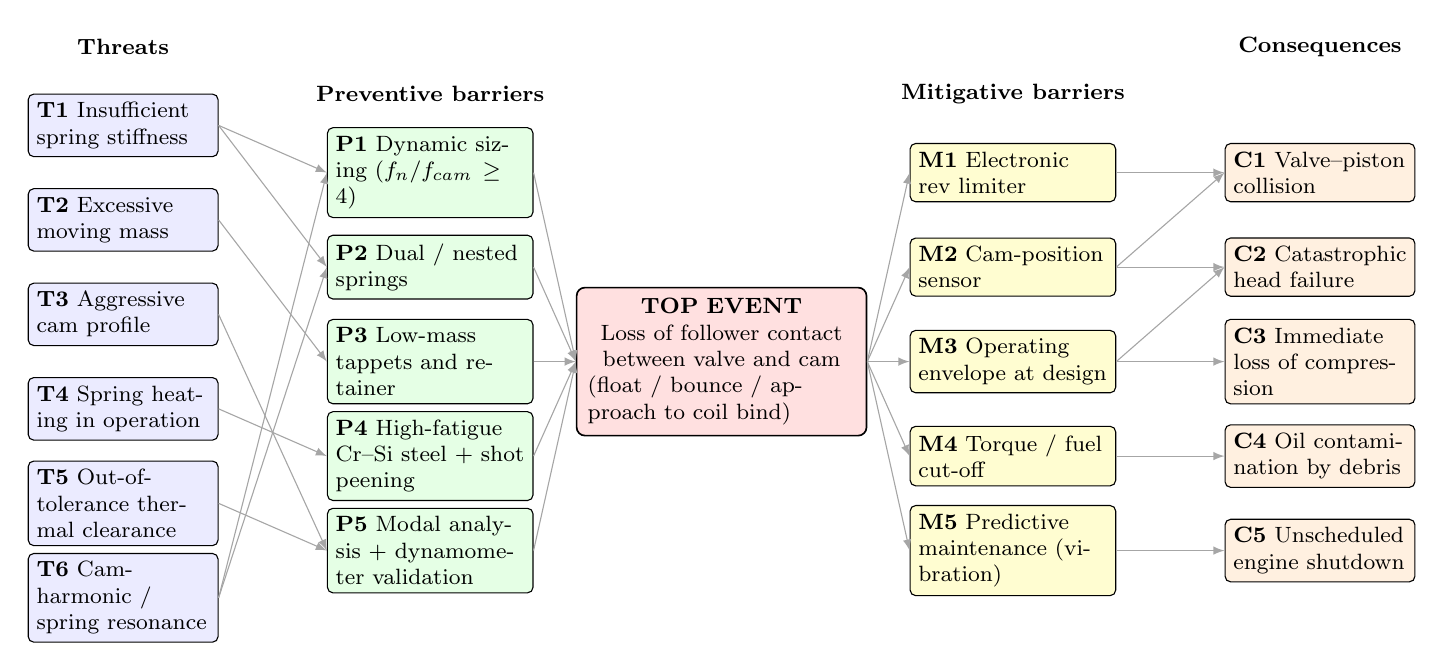
\begin{tikzpicture}[
  font=\footnotesize,
  every node/.style={align=left},
  threat/.style={draw,fill=blue!8,rounded corners=2pt,inner sep=3pt,minimum width=22mm,minimum height=6mm,text width=22mm},
  pbar/.style={draw,fill=green!10,rounded corners=2pt,inner sep=3pt,minimum width=24mm,minimum height=6mm,text width=24mm},
  cons/.style={draw,fill=orange!12,rounded corners=2pt,inner sep=3pt,minimum width=22mm,minimum height=6mm,text width=22mm},
  mbar/.style={draw,fill=yellow!18,rounded corners=2pt,inner sep=3pt,minimum width=24mm,minimum height=6mm,text width=24mm},
  topev/.style={draw,fill=red!12,line width=0.6pt,rounded corners=3pt,inner sep=4pt,minimum width=34mm,minimum height=12mm,text width=34mm},
  flow/.style={->,>=latex,line width=0.4pt,gray!70},
]

% ---- Top event (centre)
\node[topev] (TE) at (0,0)
  {\centering\textbf{TOP EVENT}\\Loss of follower contact between valve and cam\\(float / bounce / approach to coil bind)};

% ---- Threats (left, T1..T6)
\node[threat] (T1) at (-7.6, 3.0) {\textbf{T1} Insufficient spring stiffness};
\node[threat] (T2) at (-7.6, 1.8) {\textbf{T2} Excessive moving mass};
\node[threat] (T3) at (-7.6, 0.6) {\textbf{T3} Aggressive cam profile};
\node[threat] (T4) at (-7.6,-0.6) {\textbf{T4} Spring heating in operation};
\node[threat] (T5) at (-7.6,-1.8) {\textbf{T5} Out-of-tolerance thermal clearance};
\node[threat] (T6) at (-7.6,-3.0) {\textbf{T6} Cam-harmonic / spring resonance};

% ---- Preventive barriers (between threats and TE)
\node[pbar] (P1) at (-3.7, 2.4) {\textbf{P1} Dynamic sizing ($f_n/f_{cam}\geq 4$)};
\node[pbar] (P2) at (-3.7, 1.2) {\textbf{P2} Dual / nested springs};
\node[pbar] (P3) at (-3.7, 0.0) {\textbf{P3} Low-mass tappets and retainer};
\node[pbar] (P4) at (-3.7,-1.2) {\textbf{P4} High-fatigue Cr--Si steel + shot peening};
\node[pbar] (P5) at (-3.7,-2.4) {\textbf{P5} Modal analysis + dynamometer validation};

% ---- Consequences (right, C1..C5)
\node[cons] (C1) at (7.6, 2.4) {\textbf{C1} Valve--piston collision};
\node[cons] (C2) at (7.6, 1.2) {\textbf{C2} Catastrophic head failure};
\node[cons] (C3) at (7.6, 0.0) {\textbf{C3} Immediate loss of compression};
\node[cons] (C4) at (7.6,-1.2) {\textbf{C4} Oil contamination by debris};
\node[cons] (C5) at (7.6,-2.4) {\textbf{C5} Unscheduled engine shutdown};

% ---- Mitigative barriers (between TE and consequences)
\node[mbar] (M1) at (3.7, 2.4) {\textbf{M1} Electronic rev limiter};
\node[mbar] (M2) at (3.7, 1.2) {\textbf{M2} Cam-position sensor};
\node[mbar] (M3) at (3.7, 0.0) {\textbf{M3} Operating envelope at design};
\node[mbar] (M4) at (3.7,-1.2) {\textbf{M4} Torque / fuel cut-off};
\node[mbar] (M5) at (3.7,-2.4) {\textbf{M5} Predictive maintenance (vibration)};

% ---- Threats -> Preventive barriers (many-to-some mapping)
\draw[flow] (T1.east) -- (P1.west);
\draw[flow] (T2.east) -- (P3.west);
\draw[flow] (T3.east) -- (P5.west);
\draw[flow] (T4.east) -- (P4.west);
\draw[flow] (T5.east) -- (P5.west);
\draw[flow] (T6.east) -- (P1.west);
\draw[flow] (T1.east) -- (P2.west);
\draw[flow] (T6.east) -- (P2.west);

% ---- Preventive barriers -> Top event
\draw[flow] (P1.east) -- (TE.west);
\draw[flow] (P2.east) -- (TE.west);
\draw[flow] (P3.east) -- (TE.west);
\draw[flow] (P4.east) -- (TE.west);
\draw[flow] (P5.east) -- (TE.west);

% ---- Top event -> Mitigative barriers
\draw[flow] (TE.east) -- (M1.west);
\draw[flow] (TE.east) -- (M2.west);
\draw[flow] (TE.east) -- (M3.west);
\draw[flow] (TE.east) -- (M4.west);
\draw[flow] (TE.east) -- (M5.west);

% ---- Mitigative barriers -> Consequences
\draw[flow] (M1.east) -- (C1.west);
\draw[flow] (M2.east) -- (C1.west);
\draw[flow] (M3.east) -- (C2.west);
\draw[flow] (M3.east) -- (C3.west);
\draw[flow] (M4.east) -- (C4.west);
\draw[flow] (M5.east) -- (C5.west);
\draw[flow] (M2.east) -- (C2.west);

% ---- Side labels
\node[font=\footnotesize\bfseries] at (-7.6, 4.0) {Threats};
\node[font=\footnotesize\bfseries] at (-3.7, 3.4) {Preventive barriers};
\node[font=\footnotesize\bfseries] at ( 3.7, 3.4) {Mitigative barriers};
\node[font=\footnotesize\bfseries] at ( 7.6, 4.0) {Consequences};

\end{tikzpicture}
.
% =====================================================================

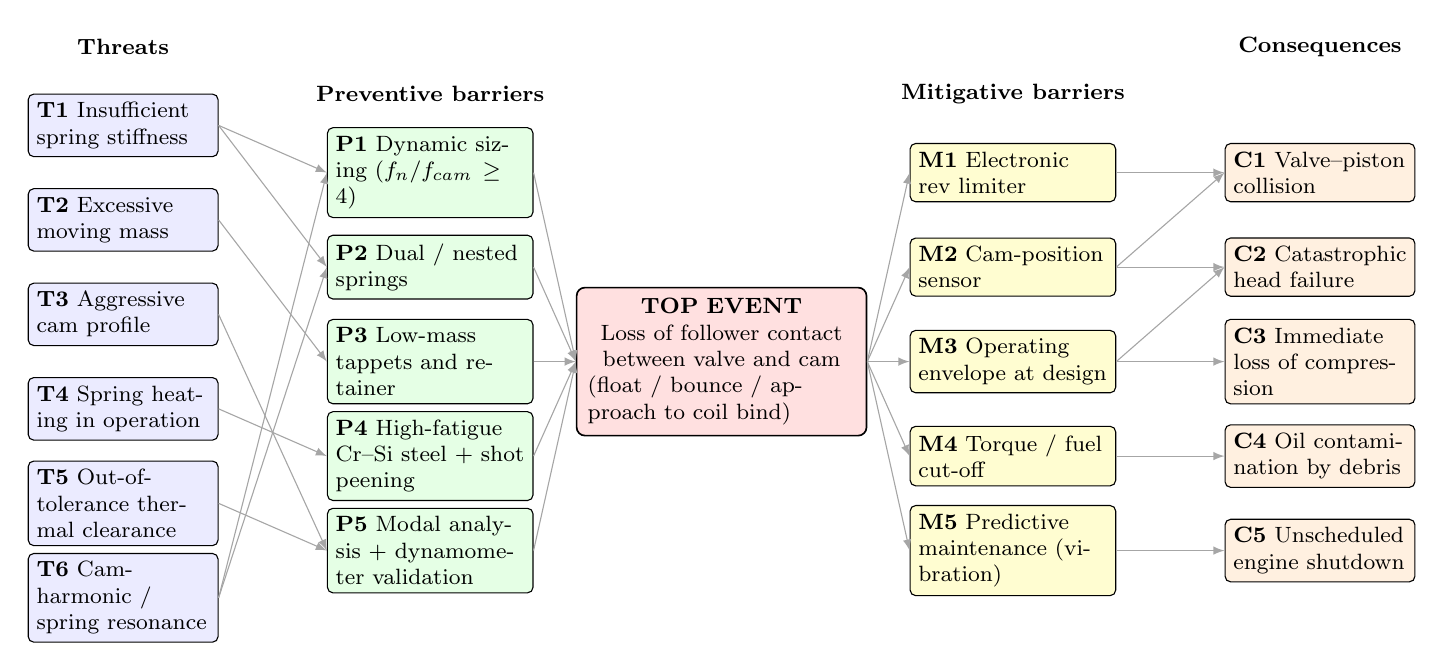
\begin{tikzpicture}[
  font=\footnotesize,
  every node/.style={align=left},
  threat/.style={draw,fill=blue!8,rounded corners=2pt,inner sep=3pt,minimum width=22mm,minimum height=6mm,text width=22mm},
  pbar/.style={draw,fill=green!10,rounded corners=2pt,inner sep=3pt,minimum width=24mm,minimum height=6mm,text width=24mm},
  cons/.style={draw,fill=orange!12,rounded corners=2pt,inner sep=3pt,minimum width=22mm,minimum height=6mm,text width=22mm},
  mbar/.style={draw,fill=yellow!18,rounded corners=2pt,inner sep=3pt,minimum width=24mm,minimum height=6mm,text width=24mm},
  topev/.style={draw,fill=red!12,line width=0.6pt,rounded corners=3pt,inner sep=4pt,minimum width=34mm,minimum height=12mm,text width=34mm},
  flow/.style={->,>=latex,line width=0.4pt,gray!70},
]

% ---- Top event (centre)
\node[topev] (TE) at (0,0)
  {\centering\textbf{TOP EVENT}\\Loss of follower contact between valve and cam\\(float / bounce / approach to coil bind)};

% ---- Threats (left, T1..T6)
\node[threat] (T1) at (-7.6, 3.0) {\textbf{T1} Insufficient spring stiffness};
\node[threat] (T2) at (-7.6, 1.8) {\textbf{T2} Excessive moving mass};
\node[threat] (T3) at (-7.6, 0.6) {\textbf{T3} Aggressive cam profile};
\node[threat] (T4) at (-7.6,-0.6) {\textbf{T4} Spring heating in operation};
\node[threat] (T5) at (-7.6,-1.8) {\textbf{T5} Out-of-tolerance thermal clearance};
\node[threat] (T6) at (-7.6,-3.0) {\textbf{T6} Cam-harmonic / spring resonance};

% ---- Preventive barriers (between threats and TE)
\node[pbar] (P1) at (-3.7, 2.4) {\textbf{P1} Dynamic sizing ($f_n/f_{cam}\geq 4$)};
\node[pbar] (P2) at (-3.7, 1.2) {\textbf{P2} Dual / nested springs};
\node[pbar] (P3) at (-3.7, 0.0) {\textbf{P3} Low-mass tappets and retainer};
\node[pbar] (P4) at (-3.7,-1.2) {\textbf{P4} High-fatigue Cr--Si steel + shot peening};
\node[pbar] (P5) at (-3.7,-2.4) {\textbf{P5} Modal analysis + dynamometer validation};

% ---- Consequences (right, C1..C5)
\node[cons] (C1) at (7.6, 2.4) {\textbf{C1} Valve--piston collision};
\node[cons] (C2) at (7.6, 1.2) {\textbf{C2} Catastrophic head failure};
\node[cons] (C3) at (7.6, 0.0) {\textbf{C3} Immediate loss of compression};
\node[cons] (C4) at (7.6,-1.2) {\textbf{C4} Oil contamination by debris};
\node[cons] (C5) at (7.6,-2.4) {\textbf{C5} Unscheduled engine shutdown};

% ---- Mitigative barriers (between TE and consequences)
\node[mbar] (M1) at (3.7, 2.4) {\textbf{M1} Electronic rev limiter};
\node[mbar] (M2) at (3.7, 1.2) {\textbf{M2} Cam-position sensor};
\node[mbar] (M3) at (3.7, 0.0) {\textbf{M3} Operating envelope at design};
\node[mbar] (M4) at (3.7,-1.2) {\textbf{M4} Torque / fuel cut-off};
\node[mbar] (M5) at (3.7,-2.4) {\textbf{M5} Predictive maintenance (vibration)};

% ---- Threats -> Preventive barriers (many-to-some mapping)
\draw[flow] (T1.east) -- (P1.west);
\draw[flow] (T2.east) -- (P3.west);
\draw[flow] (T3.east) -- (P5.west);
\draw[flow] (T4.east) -- (P4.west);
\draw[flow] (T5.east) -- (P5.west);
\draw[flow] (T6.east) -- (P1.west);
\draw[flow] (T1.east) -- (P2.west);
\draw[flow] (T6.east) -- (P2.west);

% ---- Preventive barriers -> Top event
\draw[flow] (P1.east) -- (TE.west);
\draw[flow] (P2.east) -- (TE.west);
\draw[flow] (P3.east) -- (TE.west);
\draw[flow] (P4.east) -- (TE.west);
\draw[flow] (P5.east) -- (TE.west);

% ---- Top event -> Mitigative barriers
\draw[flow] (TE.east) -- (M1.west);
\draw[flow] (TE.east) -- (M2.west);
\draw[flow] (TE.east) -- (M3.west);
\draw[flow] (TE.east) -- (M4.west);
\draw[flow] (TE.east) -- (M5.west);

% ---- Mitigative barriers -> Consequences
\draw[flow] (M1.east) -- (C1.west);
\draw[flow] (M2.east) -- (C1.west);
\draw[flow] (M3.east) -- (C2.west);
\draw[flow] (M3.east) -- (C3.west);
\draw[flow] (M4.east) -- (C4.west);
\draw[flow] (M5.east) -- (C5.west);
\draw[flow] (M2.east) -- (C2.west);

% ---- Side labels
\node[font=\footnotesize\bfseries] at (-7.6, 4.0) {Threats};
\node[font=\footnotesize\bfseries] at (-3.7, 3.4) {Preventive barriers};
\node[font=\footnotesize\bfseries] at ( 3.7, 3.4) {Mitigative barriers};
\node[font=\footnotesize\bfseries] at ( 7.6, 4.0) {Consequences};

\end{tikzpicture}
